\section{Metodologia}

\subsection{Componentes}

A metodologia escolhida para a aplicação consiste num modelo \emph{Model View Controller} (MVC), onde cada camada será responsável por uma função, sendo estas:
\begin{itemize}
    \item \emph{Views}: tudo que diz respeito a interação com usuário, ou o questionário de sintomas.
    \item \emph{Controllers}: serão responsáveis pela comunicação com os dados sobre doenças e pela aplicação de lógica sobre os sintomas apresentados pelo usuário, também como quem devolverá os possíveis passos para prevenção e tratamento para o diagnóstico, nunca deixando de reforçar a necessidade de buscar ajuda profissional.
    \item \emph{Models}: serão as entidades que representarão os dados usado pela aplicação, ou seja, as doenças, sintomas, tratamentos e talvez algum dado ainda não previsto. Ainda fará, através de classes repositórios, a persistência dos dados no banco e consultas ao mesmo.
\end{itemize}

Tais camadas sendo devidamente encapsulada e fazendo a comunicação com as outras de forma segura e sem interferir no contexto.

\begin{figure}
    \centering
    
\tikzset{every picture/.style={line width=0.75pt}} %set default line width to 0.75pt        
\resizebox{\textwidth}{!}{%
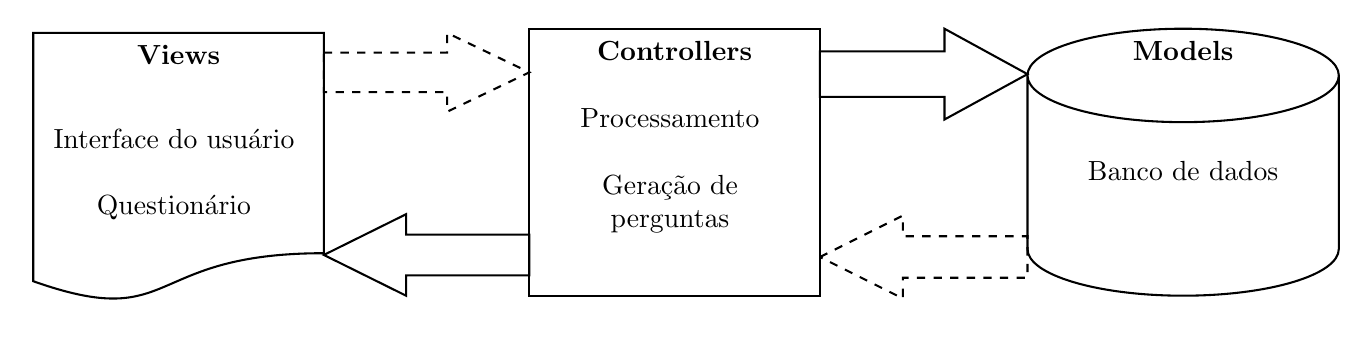
\begin{tikzpicture}[x=0.75pt,y=0.75pt,yscale=-1,xscale=1]
%uncomment if require: \path (0,300); %set diagram left start at 0, and has height of 300

%Flowchart: Magnetic Disk [id:dp16979524550945557] 
\draw (650,102.51) -- (650,186.12) .. controls (650,198.55) and (616.42,208.63) .. (575,208.63) .. controls (533.58,208.63) and (500,198.55) .. (500,186.12) -- (500,102.51)(650,102.51) .. controls (650,114.94) and (616.42,125.02) .. (575,125.02) .. controls (533.58,125.02) and (500,114.94) .. (500,102.51) .. controls (500,90.08) and (533.58,80) .. (575,80) .. controls (616.42,80) and (650,90.08) .. (650,102.51) -- cycle ;
%Flowchart: Document [id:dp9586000142466773] 
\draw (21,82.04) -- (161,82.04) -- (161,188.16) .. controls (73.5,188.16) and (91,226.42) .. (21,201.66) -- cycle ;
%Flowchart: Process [id:dp6310623690046997] 
\draw (260,80) -- (400,80) -- (400,208.63) -- (260,208.63) -- cycle ;
%Right Arrow [id:dp033275286474635735] 
\draw [dashed] (161,91.53) -- (220.4,91.53) -- (220.4,82.04) -- (260,101.02) -- (220.4,120) -- (220.4,110.51) -- (161,110.51) -- cycle ;
%Right Arrow [id:dp9102894989767911] 
\draw (400,90.94) -- (460,90.94) -- (460,80) -- (500,101.88) -- (460,123.76) -- (460,112.82) -- (400,112.82) -- cycle ;
%Left Arrow [id:dp6006547487955811] 
\draw (161,189) -- (200.6,169.38) -- (200.6,179.19) -- (260,179.19) -- (260,198.81) -- (200.6,198.81) -- (200.6,208.63) -- cycle ;
%Left Arrow [id:dp43669281204893773] 
\draw [dashed] (400,190) -- (440,170) -- (440,180) -- (500,180) -- (500,200) -- (440,200) -- (440,210) -- cycle ;

% Text Node
\draw (91,92.54) node   [align=left] {\textbf{Views}};
% Text Node
\draw (330,90.5) node   [align=left] {\textbf{Controllers}};
% Text Node
\draw (575,90.5) node   [align=left] {\textbf{Models}};
% Text Node
\draw (91,150.54) node   [align=center] {
    \begin{tabular}{c}
        Interface do usuário \\
        {}\\
        Questionário
    \end{tabular}
};
% Text Node
\draw (330,148.5) node   [align=center] {
    \begin{tabular}{c}
        Processamento\\{}\\Geração de\\perguntas
    \end{tabular}
};
% Text Node
\draw (575,148.5) node   [align=center] {Banco de dados};


\end{tikzpicture}
}
    \caption{Diagrama de blocos do sistema.}
    \label{fig:my_label}
\end{figure}

\subsubsection{Views}

Também definido como \emph{front}, ou a interface vista pelo usuário. Será estruturada como um quiz, que apresentará questões booleanas, de verdadeiro ou falso, a respeito dos sintomas do paciente.
As informações obtidas neste formulário serão enviadas para a camada \emph{Controllers}.

\subsubsection{Controllers}

Aqui ocorre a interação do banco com as informações fornecidas pelo usuário, ou seja, questões simples sobre os sintomas registrados no banco serão enviadas para o \emph{front}, em seguida, a resposta voltará para a \emph{controller}.

Baseado nisso, será realizado um mapeamento, excluindo doença que não incluem os sintomas indicados e incluindo as demais, até que o sistema aponte uma possível resposta, devolvendo para o usuário o diagnóstico, uma possível prevenção e alguma forma de tratamento.
Sempre lembrando que a avaliação de qual diagnóstico adotar será baseada num índice de incidência que está em desenvolvimento e avaliação para melhor aproveitamento, citado na subseção \ref{ssec:models}.

\subsubsection{Models}\label{ssec:models}

Consiste no banco de dados, relacionando doenças a seus sintomas e alguns possíveis tratamentos.
Pretendemos definir um valor de probabilidade para esse relacionamento, para que tenha o papel de índice de tomada de decisão para a probabilidade do usuário apresentar a doença em questão baseado neste número.
Ainda não temos plena certeza de como calcular este valor de incidência, porém algumas bibliografias apresentam dados relevantes\cite{AlbertEinstein, longo2011harrison}.

\subsection{Opções similares}

Temos como referência de aplicação o Guia de Doenças e Sintomas \cite{AlbertEinstein}, tanto como possível base de dados a ser compilados, quanto em como forma de levar o questionário ao usuário.

Apresentando informações completas, é uma excelente ferramenta para sua proposta.
Por outro lado, também ilustra o cenário que desejamos evitar, quando o usuário recebe uma lista assustadora de doenças relacionadas ao seus sintomas, tais como câncer ou insuficiência renal, quando estão ligadas ao caso por poucos sintomas.

\subsection{Avaliação e conjunto de dados}

Avaliação: A avaliação da aplicação seria feita de forma ideal recebendo respostas de um paciente e validando o diagnóstico com um médico capacitado. Embora seja possível mensurar a efetividade com casos de teste, se escolhem doenças e inserindo respostas relacionadas ao sintomas da mesma, não deixando de conferir casos excepsionais, ou  em outras palavras, casos em que o usuário possa estar com sintomas divergentes.
Podem haver testes com usuários voluntários e até opiniões médicas.

\subsection{Complementação}

Respondendo aos questionamentos deixados pelo professor, não utilizaremos sistemas de análise de linguagem natural, já que a entrada do usuário será booleana, como sim ou não.
Não encontramos nenhum módulo disponível para este sistema, mas com uma análise estatística é possível criar uma base com margem de acerto aceeitável.